\documentclass{standalone}
\usepackage{qrcode}
\usepackage{tikz}
\usepackage{xcolor}

% config following according to your wifi settings
\def\wifiname{My WiFi}
\def\wifissid{ssid here}
\def\wifipassword{mypassword}
\def\wifitype{WPA} % do not change it, if you do not know what it is
% config end

\newlength{\qrsidelen}
\setlength{\qrsidelen}{2cm}
\definecolor{midnightblue}{RGB}{25, 25, 112} % background color

\begin{document}
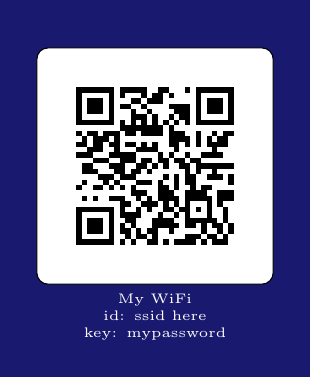
\begin{tikzpicture}
    \pagecolor{midnightblue}
    \node[draw,rounded corners,inner sep=5mm, fill=white] {
      \qrcode[height=\qrsidelen]{WIFI:T:WPA;S:\wifissid;P:\wifipassword;}
    };
    \node (pseudo) at (current bounding box.north) [inner sep=2, minimum height=5mm] {}; % for top padding
    \node[text width=3cm, text=white, font=\tiny, align=center, below] at (current bounding box.south) {\wifiname \\ id: \wifissid \\ key: \wifipassword};
  \end{tikzpicture}
\end{document}